
\providecommand{\myrootdir}{..}
\documentclass[\myrootdir/main.tex]{subfiles}

\begin{document}

\chapter{The Failing Build Logs Data Set}
\includegraphics[page=5, width=\textwidth, trim={0.5cm 0.5cm 0.5cm 0.5cm}, clip]{img/flow-of-research.pdf}

\label{sec:data-set}
\section{Motivation}
originally: log collection to get impression of build logs from various projects, what possibly extractable information they contain and how strutured or unstructured they are.
Then labeling of one build log information, namely the reason the build failed, as well as keywords and stuructural category to use in our evaluation and support our impressions about suitability of the techniques with quantitative results

\section{Related Data Sets}
\todo{kind of related work for data set? the two mortiz sent, more?}

\section{Log Collector}
To collect a broad range of build logs we built the \texttt{Log Collector} using ruby.

\subsection{Sampling Repositories}
Our first task was to determine a set of repositories to query logs from. Our \texttt{GHTorrentParser} can query the GHTorrent dataset for the most popular languages on github and the most popular repositories for a given language. \emph{Popularity} in this case is defined as the number of watches. Our \texttt{TravisRequester} can then check for a given repository whether it uses Travis CI.

\subsection{Sampling Builds}
The \texttt{LogCollector} uses the \texttt{TravisRequester}, our tool querying the Travis API, to obtain the newest builds for a given repository. As most builds on Travis CI are successful \mention{citation needed} we use a stratified sampling approach: \texttt{TravisRequester} saves the found builds in logs in buckets according to their state. We encountered the following states during our data collection passes:
\begin{itemize}
	\item \todo{fill /5 mins/}
\end{itemize}
\texttt{TravisRequester} saves up to a configured number of builds per state and searches through a configured number of maximum checked builds.

\subsection{Sampling Logs}
For each build the \texttt{TravisRequester} then selects a log to download. Logs in Travis CI are not directly attributed to \texttt{build}s, but to \texttt{job}s.
A single build can consist of multiple jobs, e.g. building and executing tests in various different testing environments.
\texttt{TravisRequester} therefore queries each build for a job, which has the same state.
A failed build can have successful job executions, as just one failed job leads to the whole build being marked as failed.
For the selected jobs, our tool then queries the Travis API V3 and obtains the respective build log.

\todo{image! like in travistorrent paper, /draft 10 mins/}

\section{Collection Process}
For our inital data collection to get an impression of build logs from various projects and languages we used the \texttt{LogCollector} to gather from the 30 most popular languages, up to 3 repositories using Travis CI each and 3 logs per state for each of those repositories.
For the \emph{Failing Build Log Data Set} we again collected from the same selection of repositories though saved only 10 logs of the state \emph{failed} for each repository.
our impression?
\todo{image!}


\section{Build Failure Reason}
\todo{WHY? one common information developers and researches might want to extract, intentionally not focus on one structurally clearly defined retrieval   cause that would be simple for PROSE retrieval -> better comparability}


\section{Data Model}
For our study, described in Chapter \ref{sec:study}, we want to investigate the retrieval capabilities of three techniques. Therefore, we need a data set of in/output examples for one \texttt{BuildLogInformation}. Furthermore, Keyword search is not configured by such in/output, but search keywords surrounding the desired output. Finally, this section describes our notion of structural categories, which we use to quantify our assumptions on the needed uniformness of in/output examples.

\subsection{Example Set}
Our data set is organized in example sets. One example set always contains build log in/output examples from the same software repository or project and for one specific build log information. They are all from one repository because we investigate information retrieval techniques which are always configured to the scope of one particular software repository or project.
Each example set has an identifying \emph{save name}, a \emph{build log information} that is desired to be extracted by this configuration, and a list of \emph{in / output examples}.

\subsection{In / Output Example}
In/output examples (I/O examples) are used to configure two of the information retrieval techniques we are evaluating for this thesis, PROSE regular expression program synthesis by example and text similarity. In our data set they always consist of an \emph{input path}, linking to the build log file which is the input for this example. The \emph{output} is a substring of that build log, the textual representation of the targeted build log information within the input build log.

\subsection{Keywords}
The keyword search is configured by a list of keywords which are searched in the document with plain text search. In order to compare it to the two other techniques, each in/output example is associated with a list of 1 - 3 keywords that can be found close to the textual representation of the targeted build log information.

\paragraph{Description}
\todo{for simple keyword search - imitate what users would search for ad-hoc}

\todo{learning steps combining keywords -> similar to how devs would learn from reading those models}

\subsection{Categories}
Our intuition was that the ability of PROSE to be able to successfully learn a regex program depended on the structural uniformity of the provided in/output examples.
The regular expressions need a consistent pattern in the build log string at the borders or around the textual representation of a build log information to match on for the retrieval.
To be able to quantify this intuition in our evaluation we assigned \emph{structural categories} to each of the examples within an example set.
If two retrievals are at the same structural location with the build log, meaning they are surrounded by a similar markings, the fall into the same category.
For most cases, two build failure reason examples which fall into one category are outputted either within the same build step or by the same build step tool.

\section{Labeling}
\subsection{Output Examples: Build Failure Reason}
We labeled the first occuring substring describing the failure. If there were multiple errors described we took the first continuous block of error description.

The labeler read or skimmed through build log and copy out the substring describing the reason the build failed. Whitespace or special characters were preserved, as they might be crucial for an information retrieval technique to detect the desired.
Because we are using xml to save our example sets, we also had to make sure to escape respective special characters (ampersand, less than).


\section{Validation}
We vaildated our collected labels in two different ways. We did a second pass of labeling the build failure reason, keywords and categoies on a subset of the data and compared the results to calculate the inter-rater reliability using cohens kappa. In addition, we sent out a survey to the developers, whose commits triggered the builds within our data set and asked them whether our retrieval of the log part describing the reason the build failed was correct. In the following we describe the results of those two validation studies.

\subsection{Inter-Rater Reliability}
re-labeling of parts of the labels - cohen's kappa

\subsection{Sending Mails to Developers}
study description \& results

\end{document}
